Классы модуля тестирования также разделены на пакеты. Отдельный пакет отведён под классы, отвечающие за использование разных языков программирования, систем оценивания, способов проверки корректности ответа, за алгоритм тестирования, за распараллеливание процесса тестирования, а также за регистрирование объектов, доступных для использования в системе, и за логирование. Схема распределения классов в модуле тестирования отображена на рис.~\ref{package_diagram_testing}.

\begin{figure}[h]
\center{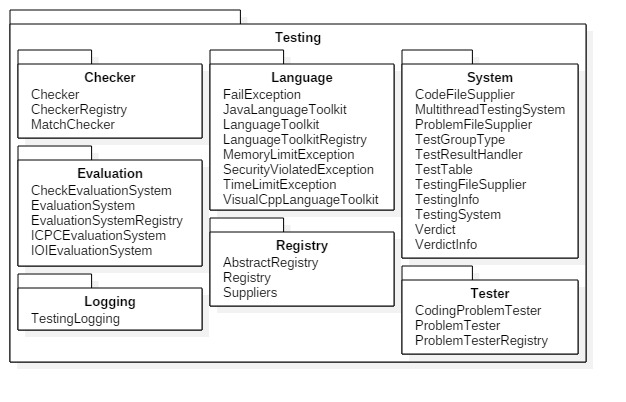
\includegraphics[scale=0.8]{package_diagram_testing}}
\caption{Модуль тестирования}
\label{package_diagram_testing}
\end{figure}

Центральное место в модуле занимают интерфейс \texttt{Testing\-System} и его реализация \texttt{Multithread\-Testing\-System}, которые принимают объекты класса \texttt{Tes\-ting\-Info} со всей необходимой информацией о посылке и ставят их в очередь на проверку. В классе \texttt{Multithread\-Testing\-System} происходит распараллеливание процесса проверки, благодаря чему каждая посылка проверяется в отдельном потоке. При этом на этапе инициализации возможно установить максимальное количество потоков, которым будет разрешено работать одновременно, так, чтобы появляющиеся новые посылки оставались в очереди и ожидали момента, когда для них освободится место. При инициализации объект этого класса также получает реализацию интерфейса \texttt{Testing\-File\-Supplier}, предоставляющего методы для работы с временными и конфигурационными файлами.

Также в системе запущен отдельный поток, в котором поочерёдно для каждой посылки после её проверки будут обрабатываться результаты посредством вызова заданной callback-функции (реализации интерфейса \texttt{Test\-Result\-Handler}). Поскольку этот процесс происходит в одном потоке, исключаются конфликты из-за конкурентного доступа в других модулях.

По окончании тестирования посылки ей присуждается некоторый вердикт с дополнительный информацией, которые записываются в объект класса \texttt{Verdict\-Info}. В нём хранится объект перечислимого типа \texttt{Verdict} (в нём перечислены все возможные вердикты, упомянутые в одной из предыдущих глав), а также максимальные время и память, затраченные решением за одном тесте, количество присуждённых очков и номер первого теста, который решение не прошло успешно, если это произошло. Такой же объект \texttt{Verdict\-Info} ставится в соответствие каждому тесту и записывается в объект класса \texttt{Test\-Table}, в котором хранится заранее подготовленная таблица с информацией о том, сколько тестов находится в каждой группе тестов.

Объект класса \texttt{Testing\-Info}, добавляемый в систему на проверку, должен быть подготовлен заранее один раз, и после отправки вызывающий код может больше не заботиться о нём. Важно только записать в него всю необходимую информацию для обработки посылки. Помимо некоторой общей информации о посылке (ограничения по времени и по памяти, которые нужно применить при тестировании, необходимости проверки только на претестах и подготовленного объекта класса \texttt{Test\-Table}) нужно также предоставить реализации следующих интерфейсов:

\begin{itemize}
\item \texttt{ProblemTester} "--- применяемый алгоритм проверки;
\item \texttt{EvaluationSystem} "--- применяемая система оценивания;
\item \texttt{LanguageToolkit} "--- выбранный язык программирования;
\item \texttt{Checker} "--- применяемый в задаче способ проверки правильности ответа;
\item \texttt{CodeFileSupplier} "--- предоставляет методы доступа к путям, по которым нужно искать файл с исходным кодом и располагать скомпилированный файл;
\item \texttt{ProblemFileSupplier} "--- предоставляет методы доступа к путям, по которым расположены тесты к задаче и скомпилированный файл чекера;
\item \texttt{TestResultHandler} "--- callback-функция для обработки результата тестирования посылки.
\end{itemize}

Рассмотрим первые четыре интерфейса более подробно. Начнём с интерфейса \texttt{Problem\-Tester}. В модуле предоставлена единственная его реализация "--- класс \texttt{Coding\-Problem\-Tester}, реализующий типичный алгоритм тестирования посылки на олимпиаде по программированию. Этот алгоритм, совмещённый с логикой системы оценивания ICPC, в общих чертах изображён на activity-диаграмме на рис.~\ref{activity_diagram_testing}. Он вполне согласуется с тем алгоритмов, что был описан в одной из предыдущих глав.

\begin{figure}[h]
\center{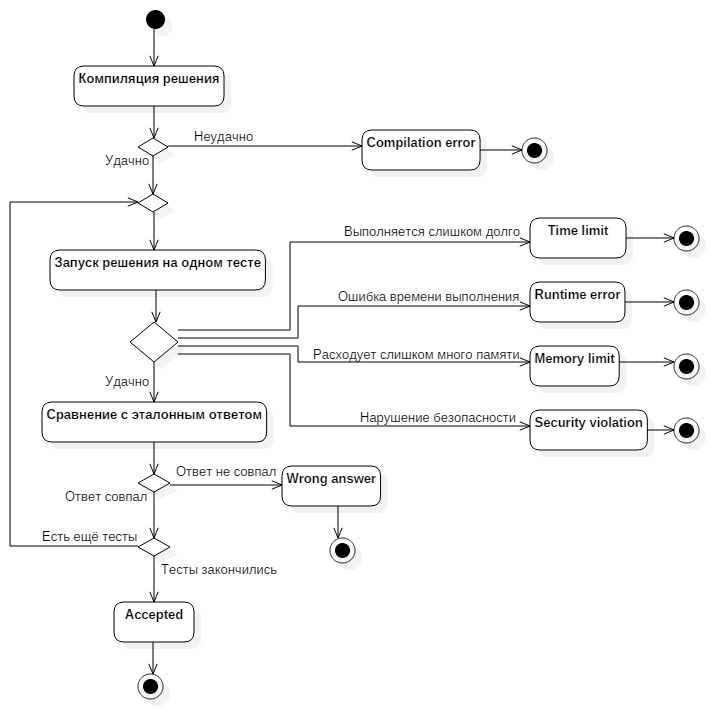
\includegraphics[scale=0.8]{activity_diagram_testing}}
\caption{Алгоритм тестирования посылки}
\label{activity_diagram_testing}
\end{figure}

Класс \texttt{Coding\-Problem\-Tester} общается с системой оценивания (реализацией интерфейса \texttt{Evaluation\-System}) посредством передачи ей объекта класса \texttt{Coding\-Tester\-Delegate} с методами для запуска тестирования посылки на определённом тесте, чтобы обеспечить системе оценивания возможность определить порядок проверки. Таким образом, поддерживается различный порядок запуска решения на тестах при разных системах оценивания.

Интерфейс \texttt{Evaluation\-System} имеет всего три метода: для определения порядка тестирования, для определения вердикта по посылке и для вычисления количества очков и штрафа по задаче на основе информации обо всех посылках, сделанных по данной задаче. В данном модуле присутствует три реализации этого интерфейса: \texttt{ICPC\-Evaluation\-System}, \texttt{IOI\-Evaluation\-System} (соответствующие двум реальным системам оценивания) и \texttt{Check\-Evaluation\-System} (специальная реализация для принудительной проверки посылки на всех тестах).

Интерфейс \texttt{Language\-Toolkit} содержит два метода: для компиляции исходного кода и для выполнения скомпилированного файла. Заметим, что именно на уровне реализаций данного интерфейса происходит отлавливание всех исключительных ситуаций, изображённых на рис.~\ref{activity_diagram_testing}. Присутствует две реализации "--- соответственно для языков Java и C++.

Класс \texttt{Java\-Language\-Toolkit} берёт из конфигурационного файла \texttt{java.pro\-perties} путь к установленному на компьютере JDK, а из файла \texttt{java\_problem.po\-licy} "--- список прав (пустой), присуждаемых запускаемым в отдельном процессе программам-решениям на языке Java. Компиляция Java-кода происходит с помощью специального API, имеющегося в JDK.

Класс \texttt{Visual\-Cpp\-Language\-Toolkit} для компиляции кода на C++ использует компилятор, поставляемый вместе со средой разработки Microsoft Visual Studio. Для этого используется конфигурационный файл \texttt{visual\_cpp.properties}. В нём прописывается путь к папке с компилятором и bat-файлом, который необходимо выполнить перед запуском компилятора. Как для компиляции, так и для выполнения скомпилированной программы запускается отдельный процесс.

Интерфейс \texttt{Checker} соответствует способу проверки правильности ответа участника на основе содержимого трёх файлов: входных данных, ответа участника и ответа жюри. По сути, он соответствует одноимённому классу из библиотеки для разработки задач, но напрямую с ним не связан (их связь реализована в модуле взаимодействия с пользователем). Зато в данном модуле есть реализация этого интерфейса по умолчанию "--- класс \texttt{MatchChecker}, "--- которая может использоваться в случаях, когда ответ в задаче единственен. Эта реализация просто проверяет на равенство ответ участника и эталонный ответ жюри.

Наконец, в данном модуле присутствует система реестров, реализующих интерфейс \texttt{Registry} и расширяющих абстрактный класс \texttt{AbstractRegistry}. Они нужны для того, чтобы хранить в них способы получения реализаций некоторых интерфейсов из данного модуля, поставленные в соответствие строковым идентификаторам. Таким образом, вызывающий код получает удобное решение в случае необходимости получить ту или иную реализацию.